\chapter{配合物的电子光谱与磁性}\label{ch:b3:complex-spectra-magnetism}

红宝石呈红色，祖母绿呈绿色，二者的颜色却都源于同一种离子，
即 \ce{Cr^{3+}}，取代了两种不同氧化物中的少量铝离子：刚玉，
$\ce{Al2O3}$，供红宝石；铍铝硅酸盐绿柱石供祖母绿。在
两者中，铬离子位于氧原子构成的八面体中；绿柱石中的
八面体略大，配体场略弱，而
离子的吸收带向红端移动约一千波数。
这足以使透射光由红变绿。本章定量阐述此类光谱：
自由离子的谱项如何在配体场中分裂，
如何借助田边–菅野图，由两个谱带位置求出
配体场分裂能与电子排斥，为何有些谱带强、
另一些弱，为何某些配合物会发生畸变，
以及磁性如何统计未成对电子。

\begin{recall}
本科二年级分册讨论了过渡元素及其 $d^n$ 组态、
晶体场分裂 $\Delta_{\mathrm o}$、高自旋与低自旋配合物、成对能、
晶体场稳定化能、$d$--$d$ 跃迁、光谱化学序列、
配体场理论，以及顺磁性和抗磁性物质。
\Cref{ch:b3:many-electron-atoms}推导了谱项符号和洪特定则，
\cref{ch:b3:group-theory-applied}讨论了约化表示与直积，
\cref{ch:b3:electronic-spectroscopy}给出了自旋选择定则与拉波特选择定则，
并描述了电荷转移跃迁，
\cref{ch:b3:partition-functions}给出了玻尔兹曼分布。
\end{recall}

\begin{omfigure}
\begin{minipage}[b]{0.3\linewidth}\centering
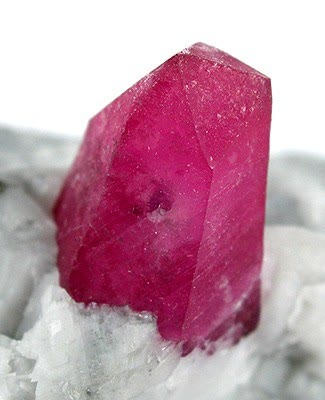
\includegraphics[height=4.2cm]{images/book4/ruby-crystal.jpg}\par
{\small 红宝石}
\end{minipage}\hspace{1.5em}
\begin{minipage}[b]{0.3\linewidth}\centering
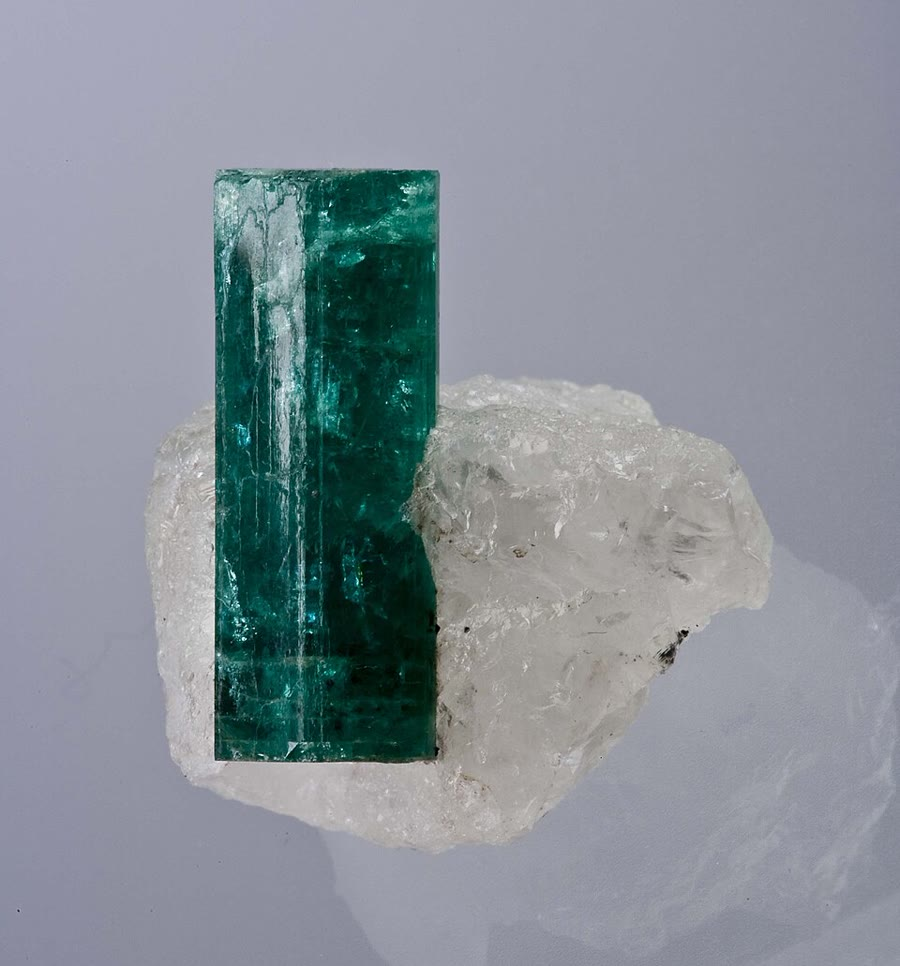
\includegraphics[height=4.2cm]{images/book4/emerald-crystal.jpg}\par
{\small 祖母绿}
\end{minipage}

{\small 一块嵌于大理石中的红宝石晶体与一块附着于石英上的祖母绿晶体。二者的
颜色均来自八面体位点中百分之几的 \ce{Cr^{3+}}。}
\end{omfigure}

\section{从自由离子谱项到配体场谱项}

在自由离子中，电子排斥将 $d^n$ 组态分裂为若干谱项
（$^4$F、$^4$P、$^2$G\dots\ 对应 $d^3$，见\cref{ch:b3:many-electron-atoms}）。在配合物中，每个谱项
还将受配体作用而进一步分裂，能级以
配合物点群的不可约表示标记。

\begin{definition}[配体场谱项]\label{def:b3:complex-spectra-magnetism:ligand-field-term}
配合物的\emph{配体场谱项}\index{配体场谱项}是指一组
简并多电子态，由其自旋多重度与
轨道部分所属点群的不可约表示标记，
例如八面体配合物中的 $^4$A$_{2g}$ 或 $^4$T$_{1g}$。
\end{definition}

\begin{proposition}[转动群的特征标]\label{prop:b3:complex-spectra-magnetism:rotation-characters}
$2L+1$ 个态，属于轨道角动量为 $L$ 的谱项，构成
转动的一个表示，对转角为 $\alpha$ 的转动，其特征标为
\[
  \chi_L(\alpha) = \frac{\sin\bigl((L + \tfrac12)\alpha\bigr)}{\sin(\alpha/2)}, \qquad \chi_L(0) = 2L + 1 .
\]
\end{proposition}

\admitted

\begin{theorem}[自由离子谱项在八面体场中的分裂]\label{thm:b3:complex-spectra-magnetism:term-splitting}
在八面体场中，$d^n$ 离子的谱项分裂为
\begin{center}
\begin{tabular}{ll}
\hline
自由离子谱项 & 八面体谱项（自旋多重度相同）\\ \hline
S & A$_{1g}$ \\
P & T$_{1g}$ \\
D & E$_g$ + T$_{2g}$ \\
F & A$_{2g}$ + T$_{1g}$ + T$_{2g}$ \\
G & A$_{1g}$ + E$_g$ + T$_{1g}$ + T$_{2g}$ \\ \hline
\end{tabular}
\end{center}
\end{theorem}

\begin{proof}
八面体群是转动群 $O$ 与反演的直积；$d$ 函数
均为偶函数，因此 $d^n$ 组态的每个谱项都是偶的（$g$），只需
在 $O$ 中约化，其类为 $E$、$8C_3$、$3C_2$ ($=C_4^2$)、$6C_4$ 和 $6C_2'$。利用
该命题，取 $L = 3$：$\chi = 7$，$\sin(420^\circ)/\sin60^\circ = 1$，$\sin(630^\circ)/\sin90^\circ = -1$，$\sin(315^\circ)/\sin45^\circ = -1$，
和 $-1$。$O$ 的特征标表（各行 $A_1$：1，1，1，1，1；$A_2$：1，1，1，$-1$，$-1$；$E$：2，
$-1$，2，0，0；$T_1$：3，0，$-1$，1，$-1$；$T_2$：3，0，$-1$，$-1$，1），以及
\cref{ch:b3:group-theory-applied}的约化公式给出 $n(A_2) = (7 + 8 - 3 + 6 + 6)/24 = 1$，$n(T_1) = (21 + 3 - 6 +
6)/24 = 1$，$n(T_2) = (21 + 3 + 6 - 6)/24 = 1$，$A_1$ 与 $E$ 的重数为零。其余各行
用同样方法求得（$L = 0$：$(1, 1, 1, 1, 1)$；$L = 1$：$(3, 0, -1, 1, -1)$；$L = 2$：$(5, -1, 1,
-1, 1)$；$L = 4$：$(9, 0, 1, 1, 1)$）。
\end{proof}

\begin{method}[自由离子谱项的分裂]\label{met:b3:complex-spectra-magnetism:split-term}
\begin{enumerate}
  \item 由洪特定则求出自由离子的基态谱项，以及
        同一多重度的激发谱项。
  \item 在表中读出它们的八面体分量，自旋多重度
        保持不变。
  \item 将其排序：对 $d^2$、$d^7$（高自旋）的基态 F 谱项，最低者为 T$_{1g}$；
        对 $d^3$、$d^8$，最低者为 A$_{2g}$（见下一命题）。
\end{enumerate}
\end{method}

\begin{proposition}[空穴与四面体反转]\label{prop:b3:complex-spectra-magnetism:hole}
八面体场中 $d^{10-n}$ 的谱项，与 $d^n$ 的谱项能量次序
相反；四面体场中 $d^n$ 的谱项，与八面体场中 $d^{10-n}$ 的谱项
相同（略去 $g$ 下标）。
\end{proposition}

\begin{proof}
$d^{10-n}$ 组态等价于满壳层中的 $n$ 个
正空穴，它们感受到的配体场势符号相反，因此每个
单电子分裂，进而每个谱项分裂，都会反号（空穴之间的
电子排斥与电子之间相同）。四面体场与八面体场的符号
相反（$e$ 轨道
能级更低），且无对称中心：$d^n$ 在 $T_d$ 中的行为如同场反号的 $d^n$，
即 $d^{10-n}$ 在 $O_h$ 中。
\end{proof}

\begin{definition}[相关图]\label{def:b3:complex-spectra-magnetism:correlation}
称\emph{相关图}\index{相关图}为一种图，它连接一个
系统在两种极限情形下的状态：弱场使自由离子谱项分裂的情形，
以及强场中组态 $t_{2g}^ae_g^b$ 的情形，连接对称性相同的状态，
且使其中任意两个状态不交叉。
\end{definition}

\begin{omfigure}
\begin{tikzpicture}[font=\small]
  % free ion
  \pic (F) at (0,0) {omlevel={}{1.1}};
  \pic (P) at (0,3.0) {omlevel={}{1.1}};
  \node[anchor=east] at (F-l) {$^3$F};
  \node[anchor=east] at (P-l) {$^3$P};
  % weak field
  \pic (a) at (2.6,-0.8) {omlevel={}{1.0}};
  \pic (b) at (2.6,0.3) {omlevel={}{1.0}};
  \pic (c) at (2.6,1.4) {omlevel={}{1.0}};
  \pic (d) at (2.6,3.1) {omlevel={}{1.0}};
  \foreach \n/\t in {a/T$_{1g}$, b/T$_{2g}$, c/A$_{2g}$, d/T$_{1g}$(P)}{\node[omsymlabel, anchor=south] at (\n-c) {$^3$\t};}
  \draw[omcorr] (F-r) -- (a-l) (F-r) -- (b-l) (F-r) -- (c-l) (P-r) -- (d-l);
  % strong field configurations
  \pic (A) at (7.4,-1.6) {omlevel={}{1.0}};
  \pic (B) at (7.4,1.4) {omlevel={}{1.0}};
  \pic (C) at (7.4,1.9) {omlevel={}{1.0}};
  \pic (D) at (7.4,4.6) {omlevel={}{1.0}};
  \node[anchor=west] at (A-r) {$^3$T$_{1g}$ \quad $t_{2g}^2$};
  \node[anchor=west] at (B-r) {$^3$T$_{2g}$};
  \node[anchor=west] at (C-r) {$^3$T$_{1g}$ \quad $t_{2g}e_g$};
  \node[anchor=west] at (D-r) {$^3$A$_{2g}$ \quad $e_g^2$};
  \draw[omcorr] (a-r) -- (A-l) (b-r) -- (B-l) (c-r) -- (D-l) (d-r) -- (C-l);
  \node[anchor=north] at (0,-2.0) {自由离子};
  \node[anchor=north] at (2.6,-2.0) {弱场};
  \node[anchor=north] at (7.4,-2.0) {强场};
  \draw[->, black!50] (3.7,-2.3) -- (6.2,-2.3) node[midway, below, font=\scriptsize] {$\Delta_{\mathrm o}$ 增大};
\end{tikzpicture}

{\small 八面体场中 $d^2$ 离子三重态的相关图。
每个弱场谱项都连接到同一对称性的强场组态，
两个 $^3$T$_{1g}$ 态不交叉：较低者连接到 $t_{2g}^2$，较高者连接到
$t_{2g}e_g$。}
\end{omfigure}

\section{田边–菅野图}

\begin{definition}[拉卡参数]\label{def:b3:complex-spectra-magnetism:racah}
称\emph{拉卡参数}\index{拉卡参数} $A$、$B$ 和 $C$ 为
由 $d$ 壳层斯莱特积分组合而成的量，它们表示所有的电子排斥
$d^n$ 组态的全部电子排斥能；同一组态各谱项之间的
能量差仅依赖于 $B$ 和 $C$，而同一最高多重度的
谱项之间的能量差仅依赖于 $B$（对 $d^2$、$d^3$、$d^7$、$d^8$：$E(\mathrm P) - E(\mathrm F) = 15B$）。
\end{definition}

\begin{example}[自由离子的拉卡参数]\label{ex:b3:complex-spectra-magnetism:free-B}
% ledger: lev:Cr3.4F5_2, lev:Cr3.4F7_2, lev:Cr3.4F9_2, lev:Cr3.4P1_2, lev:Cr3.4P3_2, lev:Cr3.4P5_2, lev:Ni2.3F3, lev:Ni2.3F2, lev:Ni2.3P2, lev:Ni2.3P1, lev:Ni2.3P0, lev:V2.4F5_2, lev:V2.4F7_2, lev:V2.4F9_2, lev:V2.4P1_2, lev:V2.4P3_2, lev:V2.4P5_2
自由 \ce{Cr^{3+}} 离子的能级中，以权重 $2J + 1$ 计算的 $^4$F 重心
在基态之上 \qty{547}{cm^{-1}}，$^4$P 在基态之上 \qty{14305}{cm^{-1}}：$15B = \qty{13758}{cm^{-1}}$，
$B = \qty{917}{cm^{-1}}$。同样的计算，\ce{V^{2+}} 得 $B = 755$，
\ce{Ni^{2+}} 得 \qty{1056}{cm^{-1}}。
\end{example}

\begin{definition}[田边–菅野图]\label{def:b3:complex-spectra-magnetism:tanabe-sugano}
称\emph{田边–菅野图}\index{田边–菅野图}为一种图，它绘出
一个 $d^n$ 离子所有配体场谱项的能量，以 $B$ 为单位，自基谱项
起算，相对于 $\Delta_{\mathrm o}/B$ 作图，且比值 $C/B$ 固定。
\end{definition}

\begin{proposition}[$d^3$ 离子的三个吸收带]\label{prop:b3:complex-spectra-magnetism:d3-bands}
在八面体场中，$d^3$ 离子自 $^4$A$_{2g}$ 出发的自旋允许跃迁位于
\[
  \nu_1 = \Delta_{\mathrm o}\ (^4\mathrm T_{2g}), \qquad
  \nu_{2,3} = 7.5B + 1.5\Delta_{\mathrm o} \mp \tfrac12\sqrt{225B^2 - 18B\Delta_{\mathrm o} + \Delta_{\mathrm o}^2}\ (^4\mathrm T_{1g}(\mathrm F), {}^4\mathrm T_{1g}(\mathrm P)).
\]
\end{proposition}

\begin{proof}[部分证明]
在强场基中，$^4$A$_{2g}$ 与 $^4$T$_{2g}$ 各出现一次，分别来自 $t_{2g}^3$ 和 $t_{2g}^2e_g$，且
二者之差不含电子排斥：$\nu_1 = \Delta_{\mathrm o}$ 精确成立。$^4$T$_{1g}$ 出现
两次，分别来自 $t_{2g}^2e_g$ 与 $t_{2g}e_g^2$；相对于 $^4$A$_{2g}$，$2\times2$ 矩阵为
$\begin{pmatrix}\Delta_{\mathrm o} + 12B & 6B\\ 6B & 2\Delta_{\mathrm o} + 3B\end{pmatrix}$（电子排斥矩阵元在本阶段不加证明地承认）。
其本征值为方程 $E^2 - (15B + 3\Delta_{\mathrm o})E + 2\Delta_{\mathrm o}^2 + 27B\Delta_{\mathrm o} = 0$ 的根，它们即
所述的 $\nu_2$ 与 $\nu_3$。当 $\Delta_{\mathrm o} = 0$ 时，它们分别为 0 与 $15B$（即 $^4$F 与 $^4$P 谱项）；完整的
对角化结果（见图）再现了它们。
\end{proof}

\begin{omfigure}
\begin{tikzpicture}
\begin{axis}[name=ta, omts, width=0.46\linewidth, height=7.0cm, xmin=1, xmax=40, ymin=0, ymax=70,
  xlabel={$\Delta_{\mathrm o}/B$}, ylabel={$E/B$}, title={\small $d^3$, $C/B = 4.5$},
  unbounded coords=jump, clip=true, clip mode=individual]
\foreach \c in {f0,f1,f2,f3,f4,f5,f6,f7,f8,f9,f10,f11,f12,f13,f14,f15}{
  \addplot[omtsforbidden, restrict x to domain=1:40] table[x=x, y=\c] {figdata/out/bachelor-3-tanabe-sugano-d3.dat};}
\foreach \c in {a0,a1,a2,a3}{
  \addplot[omDef, thick, restrict x to domain=1:40] table[x=x, y=\c] {figdata/out/bachelor-3-tanabe-sugano-d3.dat};}
\draw[omThm, dashed] (axis cs:29.0,0) -- (axis cs:29.0,70);
\draw[black!70, dashed] (axis cs:27.1,0) -- (axis cs:27.1,70);
\node[font=\scriptsize, omThm, anchor=north west, rotate=90] at (axis cs:29.6,1.5) {红宝石};
\node[font=\scriptsize, anchor=south west, rotate=90] at (axis cs:26.6,1.5) {祖母绿};
% labels outside the frame, at the height where each curve leaves it
\node[font=\scriptsize, omDef, anchor=west, inner sep=1pt] at (axis cs:40,40) {$^4$T$_{2g}$};
\node[font=\scriptsize, omDef, anchor=west, inner sep=1pt] at (axis cs:40,50.9) {$^4$T$_{1g}$};
\node[font=\scriptsize, omDef, anchor=south, inner sep=1pt] at (axis cs:32.8,70) {$^4$T$_{1g}$(P)};
\node[font=\scriptsize, black!60, anchor=west, inner sep=1pt] at (axis cs:40,21.2) {$^2$E$_g$};
\end{axis}
\begin{axis}[at={(ta.east)}, anchor=west, xshift=2.2cm, omts, width=0.46\linewidth, height=7.0cm,
  xmin=1, xmax=40, ymin=0, ymax=70, xlabel={$\Delta_{\mathrm o}/B$}, ylabel={$E/B$},
  title={\small $d^8$, $C/B = 4.71$}, unbounded coords=jump, clip=true, clip mode=individual]
\foreach \c in {f0,f1,f2,f3,f4,f5,f6}{
  \addplot[omtsforbidden, restrict x to domain=1:40] table[x=x, y=\c] {figdata/out/bachelor-3-tanabe-sugano-d8.dat};}
\foreach \c in {a0,a1,a2,a3}{
  \addplot[omDef, thick, restrict x to domain=1:40] table[x=x, y=\c] {figdata/out/bachelor-3-tanabe-sugano-d8.dat};}
\node[font=\scriptsize, omDef, anchor=west, inner sep=1pt] at (axis cs:40,40) {$^3$T$_{2g}$};
\node[font=\scriptsize, omDef, anchor=west, inner sep=1pt] at (axis cs:40,50.9) {$^3$T$_{1g}$};
\node[font=\scriptsize, omDef, anchor=south, inner sep=1pt] at (axis cs:32.8,70) {$^3$T$_{1g}$(P)};
\end{axis}
\end{tikzpicture}

{\small 对 $d^3$ 和 $d^8$ 离子，通过对该组态全部状态的配体场与电子排斥哈密顿算符
进行对角化计算得到的田边–菅野图。粗蓝线为基态多重度的各态，
粗蓝线为基态多重度的各态，
（自旋允许跃迁）；细灰线为其余各态。水平轴为基态光谱项，
（$^4$A$_{2g}$ 对应 $d^3$，$^3$A$_{2g}$ 对应 $d^8$）。虚线为红宝石和祖母绿，置于它们两条谱带的 $\Delta_{\mathrm o}/B$ 处。
$^2$E$_g$ 能级（属 $d^3$ 组态）几乎是平坦的：其能量几乎不依赖于场。}
\end{omfigure}

\begin{method}[读田边–菅野图]\label{met:b3:complex-spectra-magnetism:read-ts}
\begin{enumerate}
  \item 确定基态光谱项与自旋允许跃迁
        （多重度相同者）。
  \item 计算两谱带能量之比 $\nu_2/\nu_1$，
        并求出图中给出该比值时的 $\Delta_{\mathrm o}/B$ 值。
  \item 读取 $E/B$（对应 $\nu_1$ 处）：$B = \nu_1/(E/B)$，再求 $\Delta_{\mathrm o}$。
        对 $d^3$ 和 $d^8$，$\Delta_{\mathrm o} = \nu_1$ 直接成立；闭式公式给出 $B$，由 $\nu_2$ 计算。
  \item 将 $B$ 与自由离子的值相比较（电子云扩展比），并检验
        第三条谱带的位置是否与图中预测相符。
\end{enumerate}
\end{method}

\begin{definition}[电子云扩展效应]\label{def:b3:complex-spectra-magnetism:nephelauxetic}
\emph{电子云扩展效应}\index{电子云扩展效应}（“电子云扩展”）是指
配合物中金属离子的拉卡参数 $B$ 较自由离子的值减小，
这是由 $d$ 电子离域到配体上所引起的；
\emph{电子云扩展比}\index{电子云扩展比}为 $\beta =
B_{\text{配合物}}/B_{\text{自由离子}}$。
\end{definition}

配体成键共价性越强，$B$ 下降得越多：氟化物的 $\beta$ 约为 0.9，水的约为 0.8，
氧化物及较重卤化物约为 0.6 至 0.7，硫化物则更低。
自旋禁阻跃迁，即不同多重度光谱项之间的跃迁，
表现为弱的、常较尖锐的谱线。

\section{强度与电荷转移}

\begin{definition}[电子振动耦合]\label{def:b3:complex-spectra-magnetism:vibronic-coupling}
\emph{电子振动耦合}\index{电子振动耦合}是电子运动与振动运动的混合：
一种使配合物失去对称中心的不对称振动，
会掺入少量奇宇称（$u$）成分到其 $d$ 态中，
使拉波特禁阻的 $d$--$d$ 跃迁变为弱允许。
\end{definition}

\begin{proposition}[吸收带的强度]\label{prop:b3:complex-spectra-magnetism:intensity-order}
配合物各吸收带的摩尔吸光系数依下列顺序增大：
自旋禁阻的 $d$--$d$ $\ll$ 中心对称配合物中自旋允许的 $d$--$d$ $<$
四面体配合物中的 $d$--$d$ $<$ 电荷转移。
\end{proposition}

\begin{proof}[论证]
由\cref{ch:b3:electronic-spectroscopy}可知，跃迁在自旋守恒、宇称改变时允许。
$d$--$d$ 跃迁从不改变宇称：在八面体配合物中，它仅通过
电子振动耦合借取强度；四面体没有对称中心，其中 $d$ 轨道与 $p$ 轨道
永久混合。
自旋禁阻跃迁还借助自旋–轨道耦合再借取一小部分
强度。电荷转移跃迁使电子在金属与配体上宇称不同的轨道之间迁移，
故完全允许。
\end{proof}

\begin{definition}[电荷转移]\label{def:b3:complex-spectra-magnetism:ct}
在\emph{配体到金属的电荷转移}\index{配体到金属的电荷转移}
（LMCT）中，电子由配体轨道转移到金属轨道；
在\emph{金属到配体的电荷转移}\index{金属到配体的电荷转移}
（MLCT）中，电子由金属转移到配体的 $\pi^*$ 轨道。
\end{definition}

高锰酸根和铬酸根是 $d^0$ 离子，完全没有 $d$--$d$ 跃迁，它们的深色
源于从氧化物到空的金属 $d$ 轨道的 LMCT，这对处于高氧化态的金属很容易发生。
$\ce{[Ru(bpy)3]^{2+}}$（bpy：2,2$'$-联吡啶）的橙色则来自
由钌(II)到配体 $\pi^*$ 轨道的 MLCT 所致，该激发态即
光氧化还原催化所用的激发态（见\cref{ch:b3:photochemistry}）。在红宝石中，两条宽
带位于 560 和 \qty{410}{nm} 附近，属于
\cref{prop:b3:complex-spectra-magnetism:d3-bands}中的自旋允许 $d$--$d$ 谱带；透过的光呈红色，
并略带蓝色。受激进入这些谱带后，离子弛豫至 $^2$E$_g$ 能级，并由此
发出 \qty{695}{nm} 附近的深红色 R 线，即第一台激光器的谱线。

\section{姜–泰勒效应}

\begin{theorem}[姜–泰勒定理]\label{thm:b3:complex-spectra-magnetism:jahn-teller}
处于轨道简并电子态的非线性分子，
相对于能降低其对称性并消除简并的畸变是不稳定的。
这就是\emph{姜–泰勒定理}\index{姜–泰勒定理}。
\end{theorem}

\admitted

其对八面体配合物的推论来自各轨道的占据情况，
而 $e_g$ 轨道正指向配体。在 $d^9$ 离子（\ce{Cu^{2+}}）中，组态
$t_{2g}^6e_g^3$ 的空穴位于 $d_{z^2}$ 或 $d_{x^2-y^2}$ 中，为 E$_g$ 态。拉长两条轴向
键会使 $d_{z^2}$ 降低、$d_{x^2-y^2}$ 升高；将两个电子置于较低轨道、一个置于较高轨道，
便得到净的稳定化。铜(II)配合物确实为拉长八面体，
具有四根短键和两根长键。相同结论适用于高自旋 $d^4$（\ce{Mn^{3+}}、\ce{Cr^{2+}}）
与低自旋 $d^7$；对于 $t_{2g}$ 轨道占据不均匀的情形
（$d^1$、$d^2$、低自旋 $d^5$\dots）的轨道指向配体之间，
畸变较小。简并的激发态同样会发生畸变：
\ce{[Ti(H2O)6]^{3+}}和铜(II)配合物中宽而常为双峰的谱带，
正是其光谱特征。

\begin{omfigure}
\begin{tikzpicture}[font=\small]
  \pic[transform shape] (t) at (0,0) {omlevel={}{1.6}};
  \pic[transform shape] (e) at (0,2.2) {omlevel={}{1.1}};
  \node[anchor=east] at (t-l) {$t_{2g}$};
  \node[anchor=east] at (e-l) {$e_g$};
  \pic[transform shape] (xy) at (4.2,0.45) {omlevel={ud}{0.8}};
  \pic[transform shape] (xz) at (4.2,-0.25) {omlevel={ud}{1.4}};
  \pic[transform shape] (x2) at (4.2,3.0) {omlevel={u}{0.8}};
  \pic[transform shape] (z2) at (4.2,1.5) {omlevel={ud}{0.8}};
  \draw[omcorr] (t-r) -- (xy-l) (t-r) -- (xz-l) (e-r) -- (x2-l) (e-r) -- (z2-l);
  \node[anchor=west] at (xy-r) {$b_{2g}$ ($d_{xy}$)};
  \node[anchor=west] at (xz-r) {$e_g$ ($d_{xz}$, $d_{yz}$)};
  \node[anchor=west] at (x2-r) {$b_{1g}$ ($d_{x^2-y^2}$)};
  \node[anchor=west] at (z2-r) {$a_{1g}$ ($d_{z^2}$)};
  \node[anchor=north] at (0,-0.9) {$O_h$};
  \node[anchor=north] at (4.2,-0.9) {$D_{4h}$，拉长};
  \begin{scope}[xshift=9.0cm, yshift=1.2cm, scale=0.8]
    \pic[transform shape] {omoctahedron};
    \draw[->, thick, omThm] (0,1.25) -- (0,1.85);
    \draw[->, thick, omThm] (0,-1.25) -- (0,-1.85);
  \end{scope}
\end{tikzpicture}

{\small 一个 $d^9$ 八面体配合物的姜–泰勒畸变：拉长轴向键（右图）使 $e_g$ 分裂为 $a_{1g}$
（$d_{z^2}$，能级降低）和 $b_{1g}$（$d_{x^2-y^2}$，能级升高），$t_{2g}$ 分裂为 $e_g$ 和 $b_{2g}$。九个
电子时，单个空穴位于 $b_{1g}$ 中：畸变带来净稳定化。}
\end{omfigure}

\section{磁性}

\begin{definition}[磁化率]\label{def:b3:complex-spectra-magnetism:susceptibility}
材料的\emph{磁化率}\index{磁化率} $\chi$ 为其磁化强度与所加磁场强度之比；
\emph{摩尔
磁化率}\index{摩尔磁化率} $\chi_{\mathrm m}$ 为每摩尔的磁化率。
顺磁性物质有 $\chi > 0$，抗磁性物质则 $\chi < 0$ 且数值较小。化学上常用
$\chi_{\mathrm m}$ 的 cgs 值，单位为 \unit{cm^3.mol^{-1}}，等于国际单位制中以 \unit{m^3.mol^{-1}} 为单位的值
除以 $4\pi\times10^{-6}$。
\end{definition}

\begin{definition}[居里常数]\label{def:b3:complex-spectra-magnetism:curie}
服从居里定律的顺磁体的\emph{居里常数}\index{居里常数} $C$ 为
乘积 $\chi_{\mathrm m}T$。
\end{definition}

\begin{theorem}[居里定律]\label{thm:b3:complex-spectra-magnetism:curie}
对于自旋为 $S$、$g$ 因子为 $g$ 的独立自旋，在 $g\mu_BB \ll kT$ 的温度下，
\[
  \chi_{\mathrm m} = \frac{C}{T}, \qquad C = \frac{\mu_0N_Ag^2\mu_B^2S(S+1)}{3k}\ \ (\text{国际单位制});
\]
在 cgs 单位制中 $C = 0.1251\,g^2S(S+1)$ \unit{cm^3.K.mol^{-1}}。这就是\emph{居里定律}\index{居里定律}。
\end{theorem}

\begin{proof}[部分证明]
取 $S = \frac12$，两能级 $m_S = \pm\frac12$ 的能量为 $\pm\frac12g\mu_BB$（磁场为 $B$）。由
玻尔兹曼分布，沿磁场方向的平均磁矩为 $\frac12g\mu_B\tanh(g\mu_BB/2kT) \approx
g^2\mu_B^2B/4kT$；每摩尔的磁化强度 $M = N_Ag^2\mu_B^2B/4kT$，由 $\chi_{\mathrm m} = \mu_0M/B$ 得 $\chi_{\mathrm m} = \mu_0N_Ag^2\mu_B^2/(4kT)$，
此即取 $S(S+1) = \frac34$ 时的公式。一般情形（对 $m_S^2$ 在 $2S + 1$
个能级上取平均，$\langle m_S^2\rangle = S(S+1)/3$）在本阶段不加证明地承认。
\end{proof}

\begin{definition}[有效磁矩]\label{def:b3:complex-spectra-magnetism:moment}
顺磁性离子的\emph{有效磁矩}\index{有效磁矩}为
$\mu_{\mathrm{eff}} = \sqrt{3k\chi_{\mathrm m}T/(\mu_0N_A)}$，在 cgs 中 $\mu_{\mathrm{eff}}/\mu_B = 2.828\sqrt{\chi_{\mathrm m}T}$。其
\emph{唯自旋磁矩}\index{唯自旋磁矩}为 $2\sqrt{S(S+1)}\,\mu_B$，
即取 $g = 2$ 时仅由自旋给出的值；实测磁矩超出该值的部分，即为
\emph{轨道贡献}\index{轨道贡献}。
\end{definition}

\begin{proposition}[唯自旋公式]\label{prop:b3:complex-spectra-magnetism:spin-only}
对于 $n$ 个未成对电子，$\mu_{\text{唯自旋}} = \sqrt{n(n+2)}\,\mu_B$：1.73、2.83、3.87、4.90 和 $5.92\,\mu_B$，分别对应
$n = 1$ 至 5。
\end{proposition}

\begin{proof}
$S = n/2$，故 $2\sqrt{S(S+1)} = 2\sqrt{\frac n2(\frac n2 + 1)} = \sqrt{n(n+2)}$。
\end{proof}

\begin{proposition}[轨道贡献]\label{prop:b3:complex-spectra-magnetism:orbital-contribution}
在八面体配合物中，基谱项为 A 或 E 的离子，其磁矩接近
唯自旋值；基谱项为 T 的离子则可有相当大的
轨道贡献。
\end{proposition}

\begin{proof}[论证]
轨道磁矩需要一个轨道，它可经绕磁场轴的转动变为等价的
简并轨道，并有一个电子可在两者之间自由运动。
在 T 态（$t_{2g}$ 组不均匀填充）中，轨道 $d_{xz}$、$d_{yz}$、$d_{xy}$
经 $90^\circ$ 转动相互联系，磁矩部分保留；而在 A 态和 E 态
（$t_{2g}^3$、$t_{2g}^6e_g^2$、$e_g$ 部分填充）中，不存在这样的等价轨道，
轨道磁矩被猝灭。
\end{proof}

\begin{definition}[自旋交叉]\label{def:b3:complex-spectra-magnetism:spin-crossover}
\emph{自旋交叉}\index{自旋交叉}是配合物在
温度、压强或光照作用下，在低自旋态与高自旋态之间的转变，
当 $\Delta_{\mathrm o}$ 接近成对能时可能发生。
\end{definition}

\begin{proposition}[交叉温度]\label{prop:b3:complex-spectra-magnetism:crossover}
若转变 $\mathrm{LS} \rightleftharpoons \mathrm{HS}$ 表现为一个焓为 $\Delta H$、熵为 $\Delta S$ 的平衡，则
高自旋分数为 $x_{\mathrm{HS}} = 1/(1 + \eu^{(\Delta H - T\Delta S)/RT})$，且在 $T_{1/2} = \Delta H/\Delta S$ 时为二分之一。
\end{proposition}

\begin{proof}
$K = x_{\mathrm{HS}}/(1 - x_{\mathrm{HS}}) = \eu^{-(\Delta H - T\Delta S)/RT}$；$K = 1$ 时 $\Delta H = T\Delta S$。
\end{proof}

$\Delta H$ 与 $\Delta S$ 均为正：高自旋态的金属–配体键更长、更弱，
并有更多自旋态（由自旋单独给出的 $R\ln5$，对铁(II)，$S = 2$），因此在
高温下占优。

\begin{omfigure}
\begin{tikzpicture}
\begin{axis}[name=ct, width=0.47\linewidth, height=5.2cm, xmin=0, xmax=400, ymin=0, ymax=5.6,
  axis lines=left, xlabel={$T$ / K}, ylabel={$\chi_{\mathrm m}T$ / \unit{cm^3.K.mol^{-1}}},
  tick label style={font=\small}, label style={font=\small}]
\addplot[omDef, thick] table[x=T, y=chiT_para] {figdata/out/bachelor-3-curie-chiT.dat};
\addplot[omThm, thick] table[x=T, y=chiT_sco] {figdata/out/bachelor-3-curie-chiT.dat};
\node[font=\scriptsize, omDef, anchor=south west] at (axis cs:20,4.45) {居里顺磁体，$S = \frac52$};
\node[font=\scriptsize, omThm, anchor=west, align=left] at (axis cs:20,2.4) {自旋交叉，\\ $T_{1/2} = \qty{200}{K}$};
\end{axis}
\begin{axis}[at={(ct.east)}, anchor=west, xshift=1.5cm, width=0.47\linewidth, height=5.2cm,
  xmin=0, xmax=100, ymin=0, ymax=0.46, axis lines=left, xlabel={$1000\,\mathrm K/T$},
  ylabel={$\chi_{\mathrm m}$ / \unit{cm^3.mol^{-1}}}, tick label style={font=\small},
  label style={font=\small}]
\addplot[omDef, thick] table[x=invT, y=chi] {figdata/out/bachelor-3-curie-chi.dat};
\end{axis}
\end{tikzpicture}

{\small 左：$\chi_{\mathrm m}T$ 随 $T$ 的变化，对于居里顺磁体（$S = \frac52$，$g = 2$：恒为
\qty{4.38}{cm^3.K.mol^{-1}}）以及铁(II)自旋交叉化合物模型（$\Delta H =
\qty{15}{kJ/mol}$，$\Delta S = \qty{75}{J.K^{-1}.mol^{-1}}$），该化合物从 0（低自旋，$S = 0$）变至
\qty{3.0}{cm^3.K.mol^{-1}}（高自旋，$S = 2$）。右：居里定律，$\chi_{\mathrm m}$ 与 $1/T$ 成线性关系。}
\end{omfigure}

\begin{definition}[协同磁性]\label{def:b3:complex-spectra-magnetism:cooperative}
在\emph{铁磁性}\index{铁磁性}中，相邻顺磁中心的自旋
通过交换相互作用平行排列，从而
在居里温度以下产生自发磁化；在
\emph{反铁磁性}\index{反铁磁性}中，自旋反平行排列，
磁化率在奈尔温度以下下降。
\end{definition}

在双核配合物中，同样的交换耦合表现为 $\chi_{\mathrm m}T$ 在降温时
下降（反铁磁性）或上升（铁磁性），由此拟合出耦合
常数；桥联配体如氧化物或乙酸根通常使
金属之间呈反铁磁性耦合。

\begin{method}[用埃文斯方法测定磁矩]\label{met:b3:complex-spectra-magnetism:evans}
\begin{enumerate}
  \item 在核磁管中加入顺磁性化合物的溶液（浓度 $c$ 已知）
        及少量惰性参比物（叔丁醇，即溶剂的残留信号）；
        在同轴内管中加入相同的溶剂和参比物，
        但不含化合物。
  \item 记录 \ce{^1H} 谱：参比物给出两条谱线，间距为 $\Delta f$。
  \item 置于超导磁体中（磁场沿样品管方向），体积
        磁化率之差为 $\Delta\chi_v = 3\Delta f/f$（国际单位制，在本阶段不加证明地承认）；$\chi_{\mathrm m} = \Delta\chi_v/c$（$c$ 以
        \unit{mol.m^{-3}} 计），必要时对化合物的抗磁性作修正；
        然后求 $\mu_{\mathrm{eff}}$。
\end{enumerate}
\end{method}

\begin{inthelab}[一次埃文斯测量]
火焰封口的毛细管，或市售的同轴插件，将参比溶剂置于
核磁管内。在任何常规谱仪上，测量只需一分钟；
主要误差来自浓度和
温度，而 $\chi_{\mathrm m}$ 与 $1/T$ 成正比，因此温度必须已知。
\end{inthelab}

\begin{safety}{\ghs[0.56cm]{GHS03}\ghs[0.56cm]{GHS05}\ghs[0.56cm]{GHS06}\ghs[0.56cm]{GHS07}\ghs[0.56cm]{GHS08}\ghs[0.56cm]{GHS09}}
% ledger: ghs:K2Cr2O7
重铬酸钾以及用于电荷转移光谱的铬酸盐：
氧化剂，有毒，可能致癌并造成遗传性损伤，对
水生生物毒性极大。须在通风柜中戴手套称量；六价铬废物
需先还原，再单独收集。
\end{safety}

\begin{history}[姜与泰勒、田边与菅野]
姜和泰勒于 1937 年通过考察每一个点群证明，
轨道简并与对称的核骨架在非线性分子中互不相容。
田边和菅野于 1954 年计算了
八面体场中 $d^2$ 至 $d^8$ 离子所有谱项的能量，
方法是对与本章图中相同的矩阵作对角化；
他们的图此后一直用于指认配合物的光谱。
\end{history}

\section{练习}

\begin{exercise}[$\star$]\label{exo:b3:complex-spectra-magnetism:1}
给出 D、F、G 谱项的八面体分量，
并验证其简并度之和为 $2L + 1$。
\end{exercise}

\begin{exercise}[$\star$]\label{exo:b3:complex-spectra-magnetism:2}
对高自旋的 $d^1$ 至 $d^9$，给出自由离子的基态谱项，
以及它成为基态的八面体谱项。
\end{exercise}

\begin{exercise}[$\star$]\label{exo:b3:complex-spectra-magnetism:3}
计算高自旋的 \ce{Mn^{2+}}、\ce{Fe^{2+}} 和 \ce{Co^{2+}}，以及低自旋的
\ce{Fe^{2+}} 和 \ce{Co^{3+}} 的唯自旋磁矩。
\end{exercise}

\begin{exercise}[$\star$]\label{exo:b3:complex-spectra-magnetism:4}
将 \ce{MnO4-}、$\ce{[Mn(H2O)6]^{2+}}$、$\ce{[CoCl4]^{2-}}$ 和
$\ce{[Co(H2O)6]^{2+}}$ 的可见光吸收带按强度由小到大排序，并说明理由。
\end{exercise}

\begin{exercise}[$\star\star$]\label{exo:b3:complex-spectra-magnetism:5}
% ledger: lev:Ni2.3F3, lev:Ni2.3F2, lev:Ni2.3P2, lev:Ni2.3P1, lev:Ni2.3P0
一个镍(II)六水合配合物在 8500、14100 和 \qty{24900}{cm^{-1}} 处出现吸收带
（练习数据）。指认这些吸收带，并利用
$\nu_2 + \nu_3 = 15B + 3\Delta_{\mathrm o}$（即 $^3$T$_{1g}$ 矩阵的迹）求 $\Delta_{\mathrm o}$、$B$ 和 $\beta$（自由离子：$B = \qty{1056}{cm^{-1}}$）。
\end{exercise}

\begin{exercise}[$\star\star$]\label{exo:b3:complex-spectra-magnetism:6}
% ledger: lev:Cr3.4F5_2, lev:Cr3.4P5_2
一个铬(III)六水合配合物在 17400 和 \qty{24600}{cm^{-1}} 处有吸收
（练习数据）。求 $\Delta_{\mathrm o}$、$B$、$\beta$，并预测第三条吸收带。
\end{exercise}

\begin{exercise}[$\star\star$]\label{exo:b3:complex-spectra-magnetism:7}
红宝石和祖母绿的电子云扩展比均为 0.67，六水合铬(III)
离子为 0.79。这说明宝石中的 Cr--O 键有何特点？
\end{exercise}

\begin{exercise}[$\star\star$]\label{exo:b3:complex-spectra-magnetism:8}
判断八面体的 $d^9$、高自旋
$d^4$、低自旋 $d^7$、$d^3$、高自旋 $d^6$ 和低自旋 $d^6$ 构型的姚–泰勒畸变是强、弱还是没有。
\end{exercise}

\begin{exercise}[$\star\star$]\label{exo:b3:complex-spectra-magnetism:9}
高自旋的 \ce{Co^{2+}} 在八面体配合物中的磁矩接近 $5\,\mu_B$，
在四面体配合物中则更接近 $4.4\,\mu_B$（练习数据）。请根据基态
谱项加以解释。
\end{exercise}

\begin{exercise}[$\star\star\star$]\label{exo:b3:complex-spectra-magnetism:10}
某配合物的 $\chi_{\mathrm m}T = \qty{1.87}{cm^3.K.mol^{-1}}$，与温度无关。求 $\mu_{\mathrm{eff}}$ 及
未成对电子数。
\end{exercise}

\begin{exercise}[$\star\star\star$]\label{exo:b3:complex-spectra-magnetism:11}
在 \qty{400}{MHz}、\qty{298}{K} 下进行埃文斯测量，\qty{10.0}{mM} 的溶液使
参比信号位移 \qty{25.0}{Hz}（练习数据）。求 $\chi_{\mathrm m}$（cgs 制）及 $\mu_{\mathrm{eff}}$。
\end{exercise}

\begin{exercise}[$\star\star\star$]\label{exo:b3:complex-spectra-magnetism:12}
某自旋交叉化合物的 $\Delta H = \qty{15}{kJ/mol}$，$\Delta S = \qty{75}{J.K^{-1}.mol^{-1}}$。求 $T_{1/2}$、
\qty{250}{K} 时的高自旋分数，以及该温度下的 $\chi_{\mathrm m}T$（高自旋 $S = 2$）。
\end{exercise}

\section{问题：一个离子，两种宝石}

\begin{problem}[{周末问题——一个离子，两种宝石：铬(III)的谱项，
红宝石与祖母绿在 $d^3$ 图上的谱带，各自的配体
场与电子排斥，以及红宝石尖锐的红色谱线}]
\label{pb:b3:complex-spectra-magnetism:1}
% ledger: lf:ruby.nu1, lf:ruby.nu2, lf:emerald.nu1, lf:emerald.nu2, lf:ruby.Rline, lev:Cr3.4F5_2, lev:Cr3.4F7_2, lev:Cr3.4F9_2, lev:Cr3.4P1_2, lev:Cr3.4P3_2, lev:Cr3.4P5_2
吸收极大值（光的偏振方向垂直于晶轴）：红宝石
17\,820 和 \qty{24170}{cm^{-1}}；祖母绿为 16\,740 和 \qty{23040}{cm^{-1}}。红宝石还显示一条尖锐的
谱线，位于 \qty{695}{nm} 附近。自由 \ce{Cr^{3+}} 的 $^4$F 和 $^4$P 的重心分别位于 547 和 \qty{14305}{cm^{-1}}。

\medskip\noindent\textbf{第一部分——铬(III)。}
\begin{enumerate}
  \item 写出 \ce{Cr^{3+}} 的电子排布。
  \item 给出其自由离子的基态谱项。
  \item 在八面体场中分裂该谱项。
  \item 哪一个分支是基态谱项？为什么？
  \item $^4$P 谱项变成什么？
  \item 列出自旋允许的跃迁。
\end{enumerate}

\medskip\noindent\textbf{第二部分——谱带。}
\begin{enumerate}[resume]
  \item 将红宝石的谱带换算为波长。
  \item 将祖母绿的谱带换算为波长。
  \item 解释两种颜色。
  \item 求出每种宝石的 $\Delta_{\mathrm o}$。
  \item 为什么 $\nu_1$ 恰好等于 $\Delta_{\mathrm o}$？
\end{enumerate}

\medskip\noindent\textbf{第三部分——电子排斥。}
\begin{enumerate}[resume]
  \item 计算自由离子的 $B$。
  \item 利用 $\nu_2$ 的公式，求红宝石的 $B$（用数值方法求解）。
  \item 对祖母绿做同样的计算。
  \item 计算电子云扩展比。
  \item 计算每种宝石的 $\Delta_{\mathrm o}/B$，并将其标在图上。
  \item 预测红宝石的第三条自旋允许谱带。为什么它很少被观察到？
  \item 推测祖母绿中场为何较弱。
\end{enumerate}

\medskip\noindent\textbf{第四部分——R 线。}
\begin{enumerate}[resume]
  \item 计算 \qty{695}{nm} 处谱线的能量，以及它以红宝石的 $B$ 为单位的值。
  \item 用 $C/B = 4.5$ 绘制的图中，$^2$E$_g$ 位于 $21.0B$。
        该差值说明红宝石中的 $C/B$ 为多少？
  \item 为什么该谱线很尖锐，而谱带却很宽？
  \item 为什么发射过程很慢？
  \item 为什么该谱线在祖母绿中应位于几乎相同的位置？
  \item 为什么寿命较长的激发态能使激光成为可能？
  \item 给出结果：$\Delta_{\mathrm o}(\text{红宝石}) - \Delta_{\mathrm o}(\text{祖母绿})$ 的差值。
\end{enumerate}
\end{problem}
